\documentclass[11pt]{report}
\usepackage[a4paper]{geometry}
\usepackage[myheadings]{fullpage}
\usepackage{fancyhdr}
\usepackage{lastpage}
\usepackage{graphicx, wrapfig, subcaption, setspace, booktabs}
\usepackage[T1]{fontenc}
\usepackage[font=small, labelfont=bf]{caption}
\usepackage[protrusion=true, expansion=true]{microtype}
\usepackage{sectsty}
\usepackage{url, lipsum}
\usepackage{mathptmx}
\usepackage[utf8]{inputenc}
\usepackage[francais]{babel}
\pagestyle{plain}

\newcommand{\HRule}[1]{\rule{\linewidth}{#1}}
\onehalfspacing
\setcounter{tocdepth}{5}
\setcounter{secnumdepth}{5}

\renewcommand{\thesection}{\arabic{section}}

%-------------------------------------------------------------------------------
% TITLE PAGE
%-------------------------------------------------------------------------------

\begin{document}

\title
{
	\Large{Projet de communication transdisciplinaire}
	\HRule{2pt} \\ [0.5cm]
	\LARGE \textbf{\uppercase{Bacchanight}}
	\HRule{2pt} \\ [0.5cm]
	\normalsize \today
}

\date{}

\author
{
	\LARGE{Université de Bordeaux} \\
	\\
	Guillaume CHARLET \\
    Kenji FONTAINE \\
    Gauthier LAMARQUE \\
}

\maketitle

%-------------------------------------------------------------------------------
% Présentation du projet
%-------------------------------------------------------------------------------

\renewcommand{\thesection}{\arabic{section}}

\section{Présentation du projet}

La Baccha-night, du mot « bacchanales », fêtes mythologiques en l’honneur du
dieu du vin Bacchus, est un évènement nocturne étudiant proposé par le musée
des Beaux-Arts de Bordeaux le mardi 21 mars 2017.
Le but de ce projet est d'élaborer un outil permettant de mieux renseigner
les internautes sur la soirée (programme, accès, réseaux sociaux, etc.). \\
Ce projet a été mené sur l'ensemble de l'année scolaire 2016/2017. Les membres
composants l'équipe a pu changer au cours de l'année. De ce fait, le rapport est
divisé en deux parties, une pour chaque semestre.

\section{Premier semestre}

L'équipe est initialement composé de :
\begin{itemize}
 	\item Julien COUVY
    \item Kenji FONTAINE
    \item Gauthier LAMARQUE
    \item Enzo PERUZZETTO
	\item Guillaume CHARLET (qui nous rejoindra un peu plus tard)
\end{itemize}

\subsection{Déroulement}

Pour les premières séances, notre priorité était d'avoir une idée claire
de ce que nous devions faire. Nous avons alors commencé par nous renseigner sur
ce qu'était la Bacchanight. Après une séance de recherche et de mise en commun,
nous avons vu, qu'en effet les informations étaient difficiles à trouver.
\par
Nous nous sommes alors demandé quelle forme pourrait prendre un outil numérique
permettant une bonne transmission des informations. Finalement, nous avons décidé
que faire un site web dédié à la soirée serait une bonne solution. \\
Ensuite, nous avons regardé différents sites présentant des événements similaires
à la Bacchanight afin d'avoir une meilleure idée de ce qui était attendu d'un
tel site. Suite à cette recherche, le modèle "Page unique" ou "One Page" a été
retenu de par sa simplicité et son efficacité. \\
C'est à ce moment que \textit{Guillaume Charlet} a rejoint notre équipe.
\par
Le prochain objectif pour notre groupe était alors de mettre sur papier,
la forme qu'allait prendre notre page. Barre de navigation, boutons,
système utilisateurs, système permettant de commenter, photos, vidéos, carousel... \\
Le prototype ainsi obtenu est disponible en annexe.

\subsection{Choix des technologies}

Afin de faciliter le déploiment et la mise en ligne de notre travail, utiliser la
même technologie que le site actuel du Musée des Beaux Arts est le plus simple.
Nous avons ainsi décider d'utiliser le même système de gestion du contenu
\textbf{Drupal 7}. \\
Cela ajoute une nouvelle difficulté au projet: Notre produit doit être facilement
exportable, afin que la mise en ligne de la page web soit réalisable.

Le site doit permettre l'accès aux informations suivantes :
\begin{itemize}
	\item Description de la soirée,
	\item Date et lieu,
	\item Programme de la soirée,
	\item Photos de l'événement,
	\item Remerciements et Partenaires,
	\item Contact, lien vers les réseaux sociaux du Musée des Beaux Arts.
\end{itemize}

\vspace{0.5cm}

\section{Second semestre}

Au départ de ce second semestre, nous n'étions plus que 3 à continuer ce projet.
Un second groupe a décidé de réaliser le même projet que nous. Conjointement,
et avec l'approbation de M. Blin, il a été convenu que chaque groupe devrait
réaliser une version statique du site que nous souhaiterions réaliser, en se
détachant totalement du CMS Drupal. Le but de cette démarche était de proposer au
Musée des Beaux Arts deux versions du site, et que l'une des ces deux versions serait
choisie pour que nous puissions travailler efficacement sur celle-ci.\\
Vous pouvez retrouvez la version retenue à l'adresse suivante:

\vspace{0.5cm}

\textbf{mba.emi.u-bordeaux.fr}\\

\par
Il s'agit du site statique proposé par l'autre groupe, vous pouvez en voir un
aperçu en annexe 2. Dès lors que le choix de l'apparence du site était fixé,
nous nous sommes plongés sur les différentes tâches inhérentes aux besoins
fonctionnels du site, tout en essayant de rester au plus proche de l'aspect
graphique retenu.

\newpage
\section{Champs modifiables}

\subsection{Couleur principale}

La couleur principale est décrite par un champ texte d'une longueur maximale de
7 caractères. La couleur est exprimée en hexadécimal de la façon suivante :
\textbf{\#000000} à \textbf{\#FFFFFF}. \\
Cette couleur est utilisée pour les éléments suivants de la page :
\begin{itemize}
	\item La mise en valeur d'un élément dans la barre de navigation.
	\item Le bouton "Découvrez Bacchanight!" inclus dans l'image d'en-tête.
	\item L'écriture des balises \textbf{[G]} et \textbf{[M]} indiquant le lieu d'un événement dans le programme.
	\item Le bouton "Envoyer" dans la section \textbf{Contact}.
	\item L'écriture des catégories d'informations en bas de page.
	\item La partie basse de l'effet dégradé en bas de page.
\end{itemize}

\subsection{Couleur secondaire}

La couleur secondaire est définie de la même façon que la couleur principale.
Cette couleur est utilisée pour l'élément suivant de la page :
\begin{itemize}
	\item La partie haute de l'effet dégradé en bas de page.
\end{itemize}

\subsection{Image fond}

L'image de fond est utilisé comme image d'en-tête. Elle est également utilisé
pour les bannières \textbf{Programme}, \textbf{Galerie}, \textbf{Contact} et
\textbf{Partenaires}. L'effet de bichromie n'est pas obtenu automatiquement , il
est nécessaire de le faire à la main. \\
Ce champ image est stocké et est modifiable via Drupal. \\
Les extensions suivantes sont acceptées : \textbf{png, gif, jpg, jpeg}.

\subsection{Image description}

Cette image est affichée à gauche du texte de description. Lorsqu'un utilisateur
passe son curseur sur l'image, celle-ci passe en couleur. Cet effet est automatique.
Ce champ image est stocké et est modifiable via Drupal. \\
Les extensions suivantes sont acceptées : \textbf{png, gif, jpg, jpeg}.

\subsection{Description}

La description de la soirée est un champ texte long géré par Drupal.
Seules les balises HTML suivantes autorisées : \textbf{<strong> <br> <p>}.

\subsection{Programme}

Le programme est généré à partir d'un fichier texte que l'administrateur
téléchargera vers du pannel d'administration de Drupal. \\
Une seule extension de fichier est acceptée : \textbf{txt}.
Le fichier txt devra être rédigé de la façon suivante :
\begin{verbatim}
	l.1 Horaires de l'événement 1 (\textbf{ex :} 00h00 à 23h59)
	l.2 Titre de l'événement 1
	l.3 Description de l'événement 1 (Ne pas revenir à la ligne avec entrée, même si la description fait plus d'une ligne.)
	l.4 Emplacement de l'événement 1 G ou M (Les [ ] sont mises automatiquement.)
	l.5 (Laisser une ligne vide)
	l.6 Horaires de l'événement 2
	l.7 Titre de l'événement 2
	l.8 etc...
\end{verbatim}

\subsection{Image Programme}

Cette image est affichée à droite de la section \textbf{Programme}. De même que
pour \textbf{l'Image Description}, l'effet couleur est automatique.
Ce champ image est stocké et est modifiable via Drupal. \\
Les extensions suivantes sont acceptées : \textbf{png, gif, jpg, jpeg}.

\subsection{En continu}

La section \textbf{En continu} est géré de la même façon que le \textbf{Programme}.
Les fichiers texte générant ces deux sections utilisent la même syntaxe et se
rédigent de la même façon. Un fichier correspond à une seule section du Programme.
Il faut donc deux fichiers texte, un pour le "Programme" et un pour le "En continu".
De même que pour le programme, seul l'extension \textbf{txt} est acceptée.

\subsection{Galeries}

Ces images seront affichées dans la section \textbf{Galeries} du site. Elles sont
stockées dans un champ image de Drupal dans lequel il est possible de télécharger
individuellement plusieurs images, avec une limite de 10 images maximum.
Il est possible de les réordonner ou supprimer individuellement. \\
Les extensions suivantes sont acceptées : \textbf{png, gif, jpg, jpeg}.

\subsection{Captcha Key}

Il s'agit d'une chaîne de caractères permettant de sécuriser l'envoi du formulaire
de contact. Cette clé doit provenir de l'API reCaptcha de Google. Cela permet de
prévenir de potentielles intrusions de bots, et assurer le bon fonctionnement
de l'envoi de formulaire au Musée des Beaux Arts de Bordeaux présent dans la
section \textbf{Contact} du site.\\
Tout cela est stocké dans un le champ texte de Drupal dont la longueur maximale
est de 255 caractères.

\subsection{Texte partenaire}

Le texte de remerciements des partenaires est affiché dans la section
\textbf{Contact} du site. Il est stocké dans un champ texte long par Drupal. \\
Le texte est traité tel quel, aucune balise HTML n'est acceptée.

\subsection{Image partenaire}

Cette image est affichée dans la section \textbf{Contact} du site. Elle se place
juste en-dessous du texte destiné aux remerciements des partenaires.
L'image est stockée dans un champ image de Drupal. \\
Les extensions suivantes sont acceptées : \textbf{png, gif, jpg, jpeg}.

\subsection{Date et heure}

La description de la soirée est un champ texte stocké par Drupal, dont la longueur
maximale est de 30 caractères. Le texte est traité tel quel, l'affichage dépendra
de la façon dont l'administrateur Drupal l'a défini. \\
\textbf{exemple :} DD/MM/YYYY ou Day DD Month YYYY


L'heure est également stocké dans un champ texte géré par Drupal. La longueur
maximale est de 25 caractères. Le texte est traité tel quel, l'affichage dépendra
de la façon dont l'administrateur Drupal l'a défini. \\
\textbf{exemple :} HH : MM - HH : MM

\subsection{Contact téléphone}

Le numéro de téléphone de contact est affiché dans la partie informations de
contact dans la section \textbf{Contact}, en bas de page.
Le numéro de téléphone est stocké dans un champ texte par Drupal, d'une taille
maximale de 20 caractères. Il s'agit de texte simple, aucune balise HTML est autorisée.

\subsection{Contact mail}

L'adresse mail de contact est affichée dans la partie informations de
contact dans la section \textbf{Contact}, en bas de page.
L'adresse mail de contact est stockée dans un champ texte par Drupal, d'une taille
maximale de 255 caractères. Il s'agit de texte simple, aucune balise HTML est autorisée.

\subsection{Réseaux sociaux}

Chaque réseau social est stocké de manière individuelle dans un champ texte de
Drupal (255 caractères au maximum). Chaque champ texte correspond à un réseau
social : Facebook, Twitter et Instagram. Ces champs texte correspondent aux liens
vers les réseaux sociaux du Musée des Beaux Arts. \\
\textbf{exemple : } https://www.facebook.com/bordeaux.musee.ba

\subsection{Copyright}

Le texte de copyright est affiché tout en bas de page.
Il est stocké dans un champ texte par Drupal, d'une taille maximale de 255
caractères. Il s'agit de texte pur, aucune balise HTML est autorisée.

%-------------------------------------------------------------------------------
% jdeploi
%-------------------------------------------------------------------------------

\subsection*{Déploiement}
La procédure de déploiement est explicitée en détails dans le fichier
suivant : \textbf{deploiement.pdf}

%-------------------------------------------------------------------------------
% Besoins non fonctionnels
%-------------------------------------------------------------------------------

\section{Besoins non fonctionnels}

\subsection*{Charte graphique}

La charte graphique est fournie par le Musée des Beaux Arts de Bordeaux. Elle définit
les couleurs, polices utilisées pour le site. Ces paramètres sont modifiables par
l'intermédiaire de Drupal. \\
Le site est sous un format One Page. Un site One Page est un site constitué
d'une seule et même page sur laquelle l'ensemble des informations du site
est disponible en scrollant (ou à l'aide d'une barre de navigation).

\subsection*{Accessibilité}

Le site doit être accessible à partir des navigateurs suivants (toutes plateformes confondues):
\begin{center}
	\begin{tabular}{|l | r|}
		\hline
		Navigateurs & Parts de marché \\
		\hline
		\hline
		Google Chrome 54+ & 51\% \\
		\hline
		Mozilla Firefox 51.0+ & 7,4\% \\
		\hline
		Safari (Apple) 10.0+ & 18,3\% \\
		\hline
		Microsoft Edge / IE 11.0 & 10,8\% \\
		\hline
	\end{tabular}
\end{center}
Ces navigateurs ont été sélectionnés à partir de leur pourcentage de parts de
marché (toutes supérieures à 5\%). Ce pourcentage est une moyenne des pourcentages
recueillis sur les sites suivants:
\begin{itemize}
	\item StatCounter
	\item Net MarketShare
	\item W3Counter
	\item Akamai
\end{itemize}

\subsection*{Responsive}
Le site doit être accessible depuis plusieurs plateformes, le site doit s'adapter
à la taille de l'écran.

%-------------------------------------------------------------------------------
% Retro planning
%-------------------------------------------------------------------------------

\section{Retro planning}

\begin{itemize}
	\item Septembre 2016 : Création des groupes, choix du projet.
	\item Octobre/Novembre 2016 : Conception et choix des technologies.
	\item Décembre 2016 : Prise en main de Drupal, création d'une maquette.
	\item Janvier 2017 : Approfondissement de l'utilisation de Drupal.
	\item Février/Mars 2017 : Développement de la version statique du site.
	\item Avril 2017 : Développement de la version sous Drupal en vue d'un déploiement.
\end{itemize}

%-------------------------------------------------------------------------------
% Maquette
%-------------------------------------------------------------------------------

\newpage

\section*{Annexe 1 : Maquette du premier semestre}

\vspace{0.4cm}
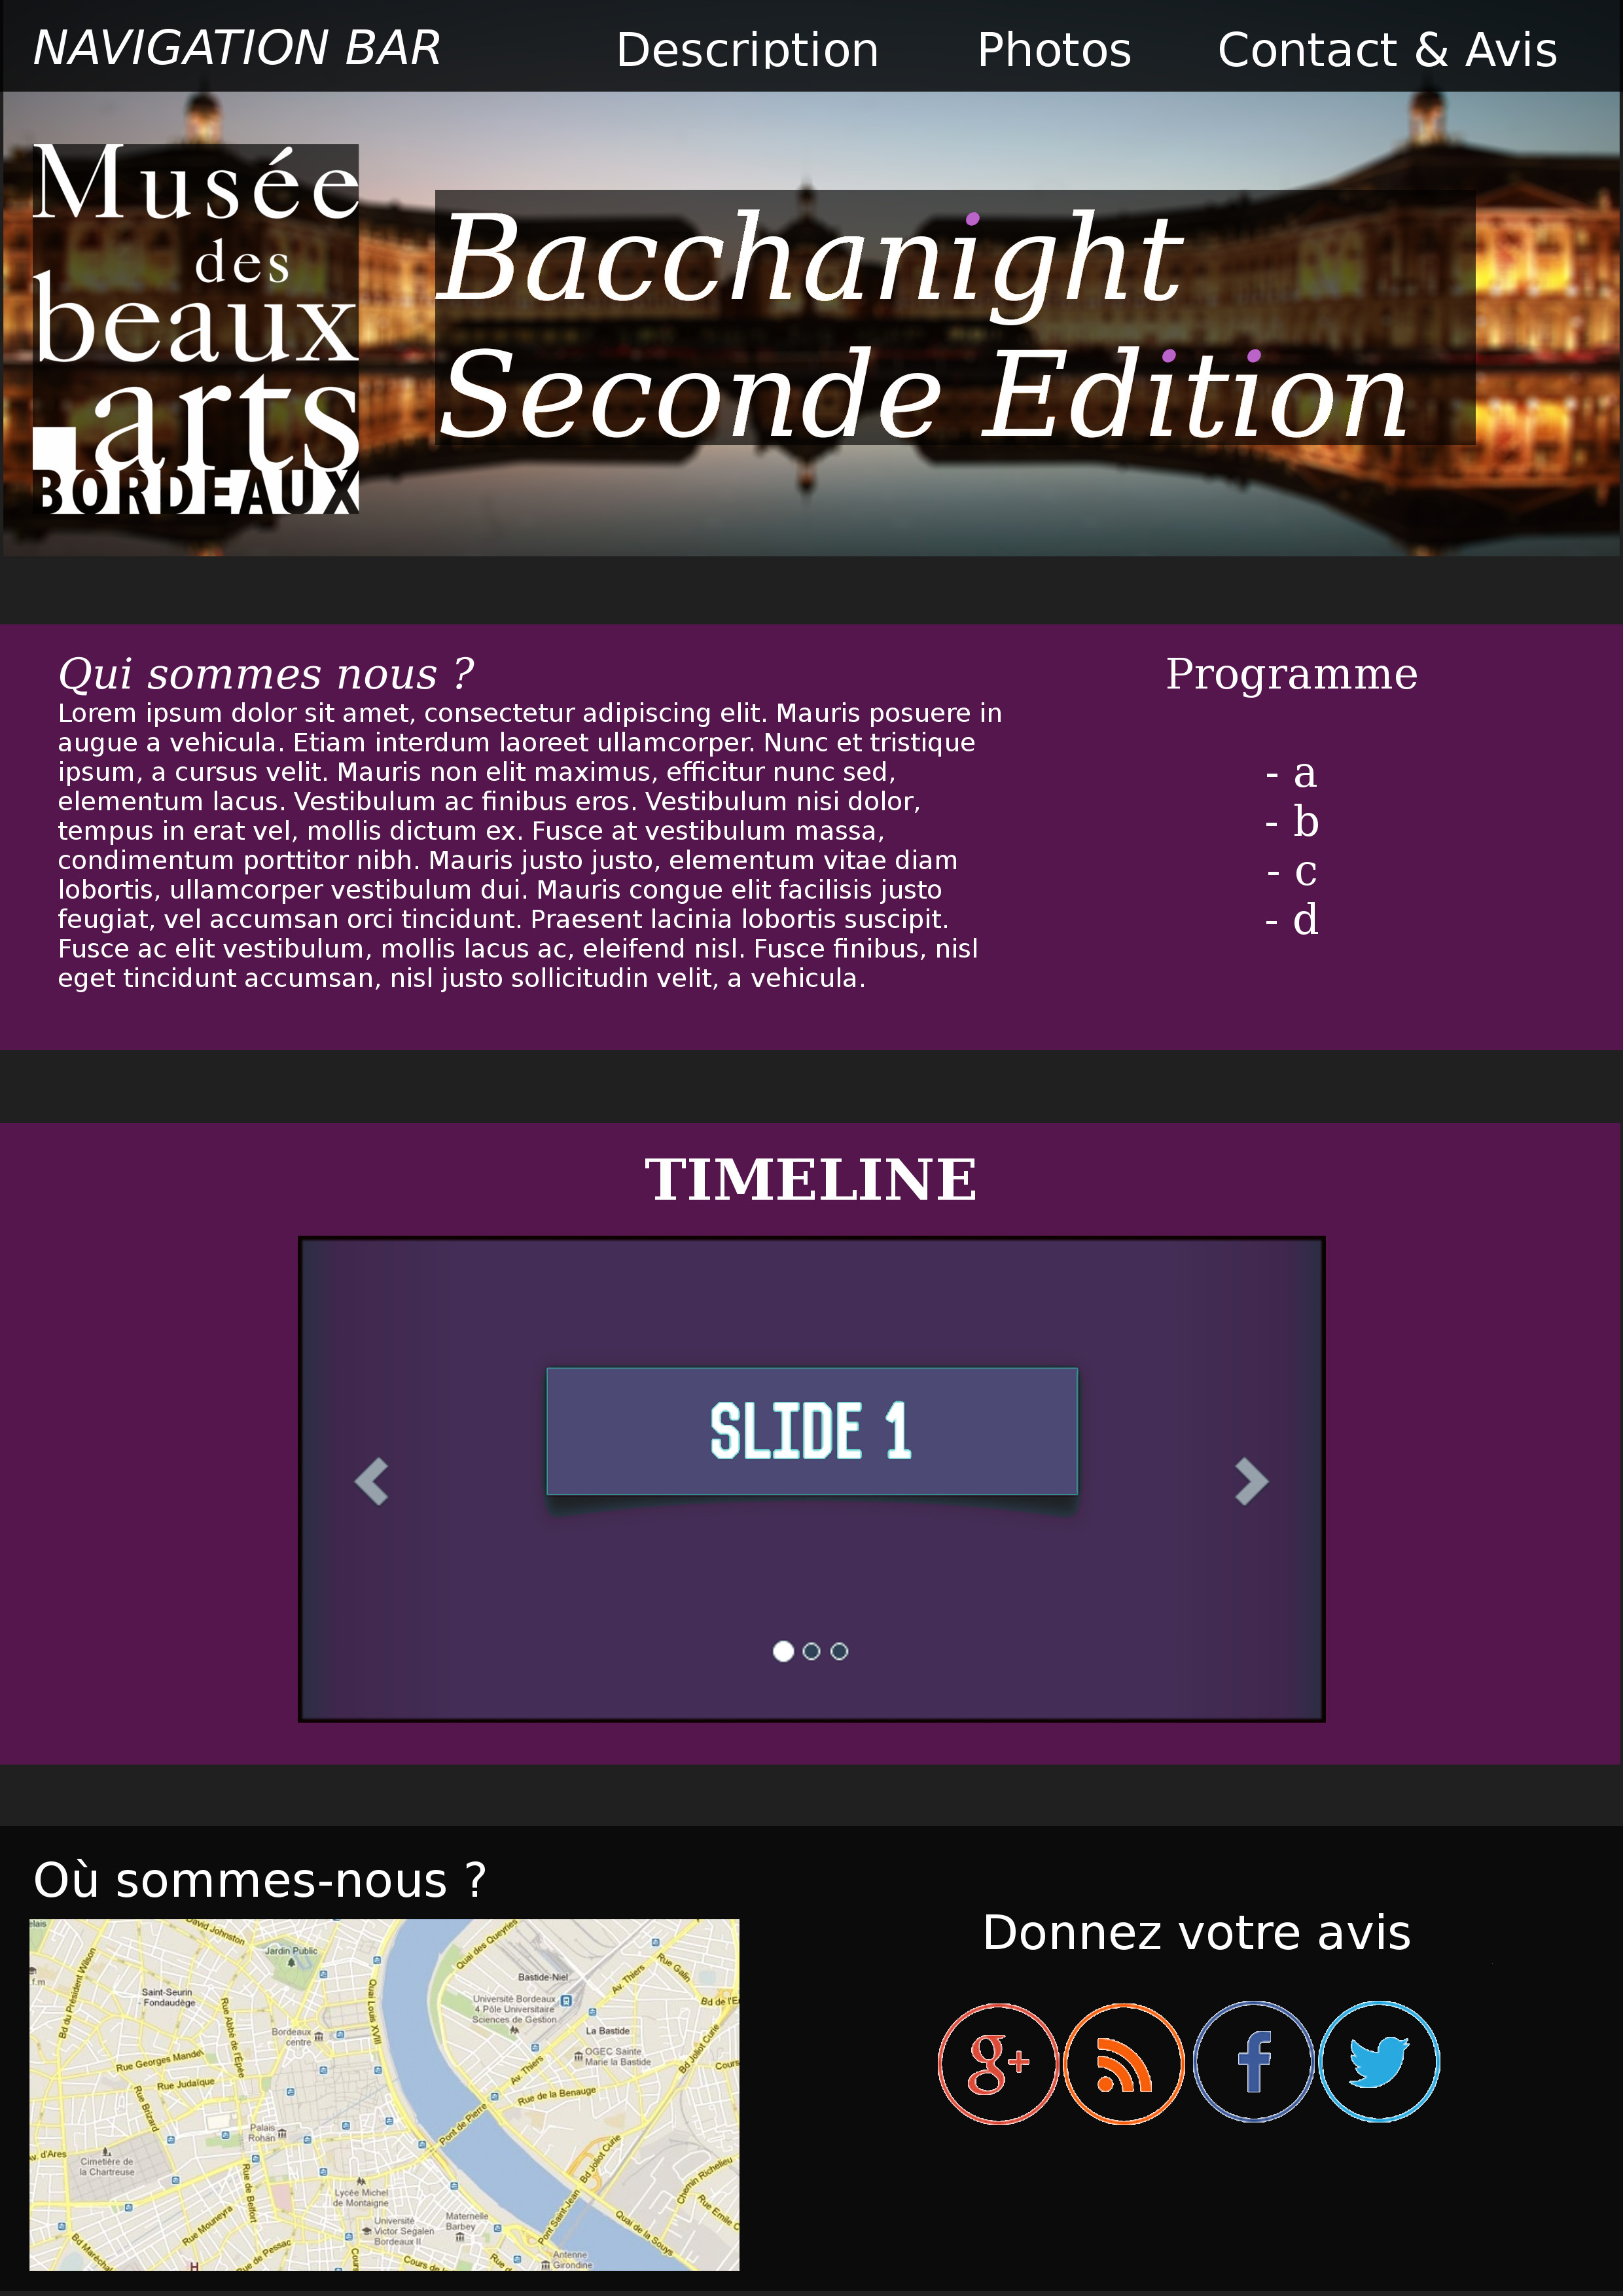
\includegraphics[scale=0.75]{maquette.jpg}

\section*{Annexe 2 : Aperçu du site statique retenu}

\vspace{0.4cm}
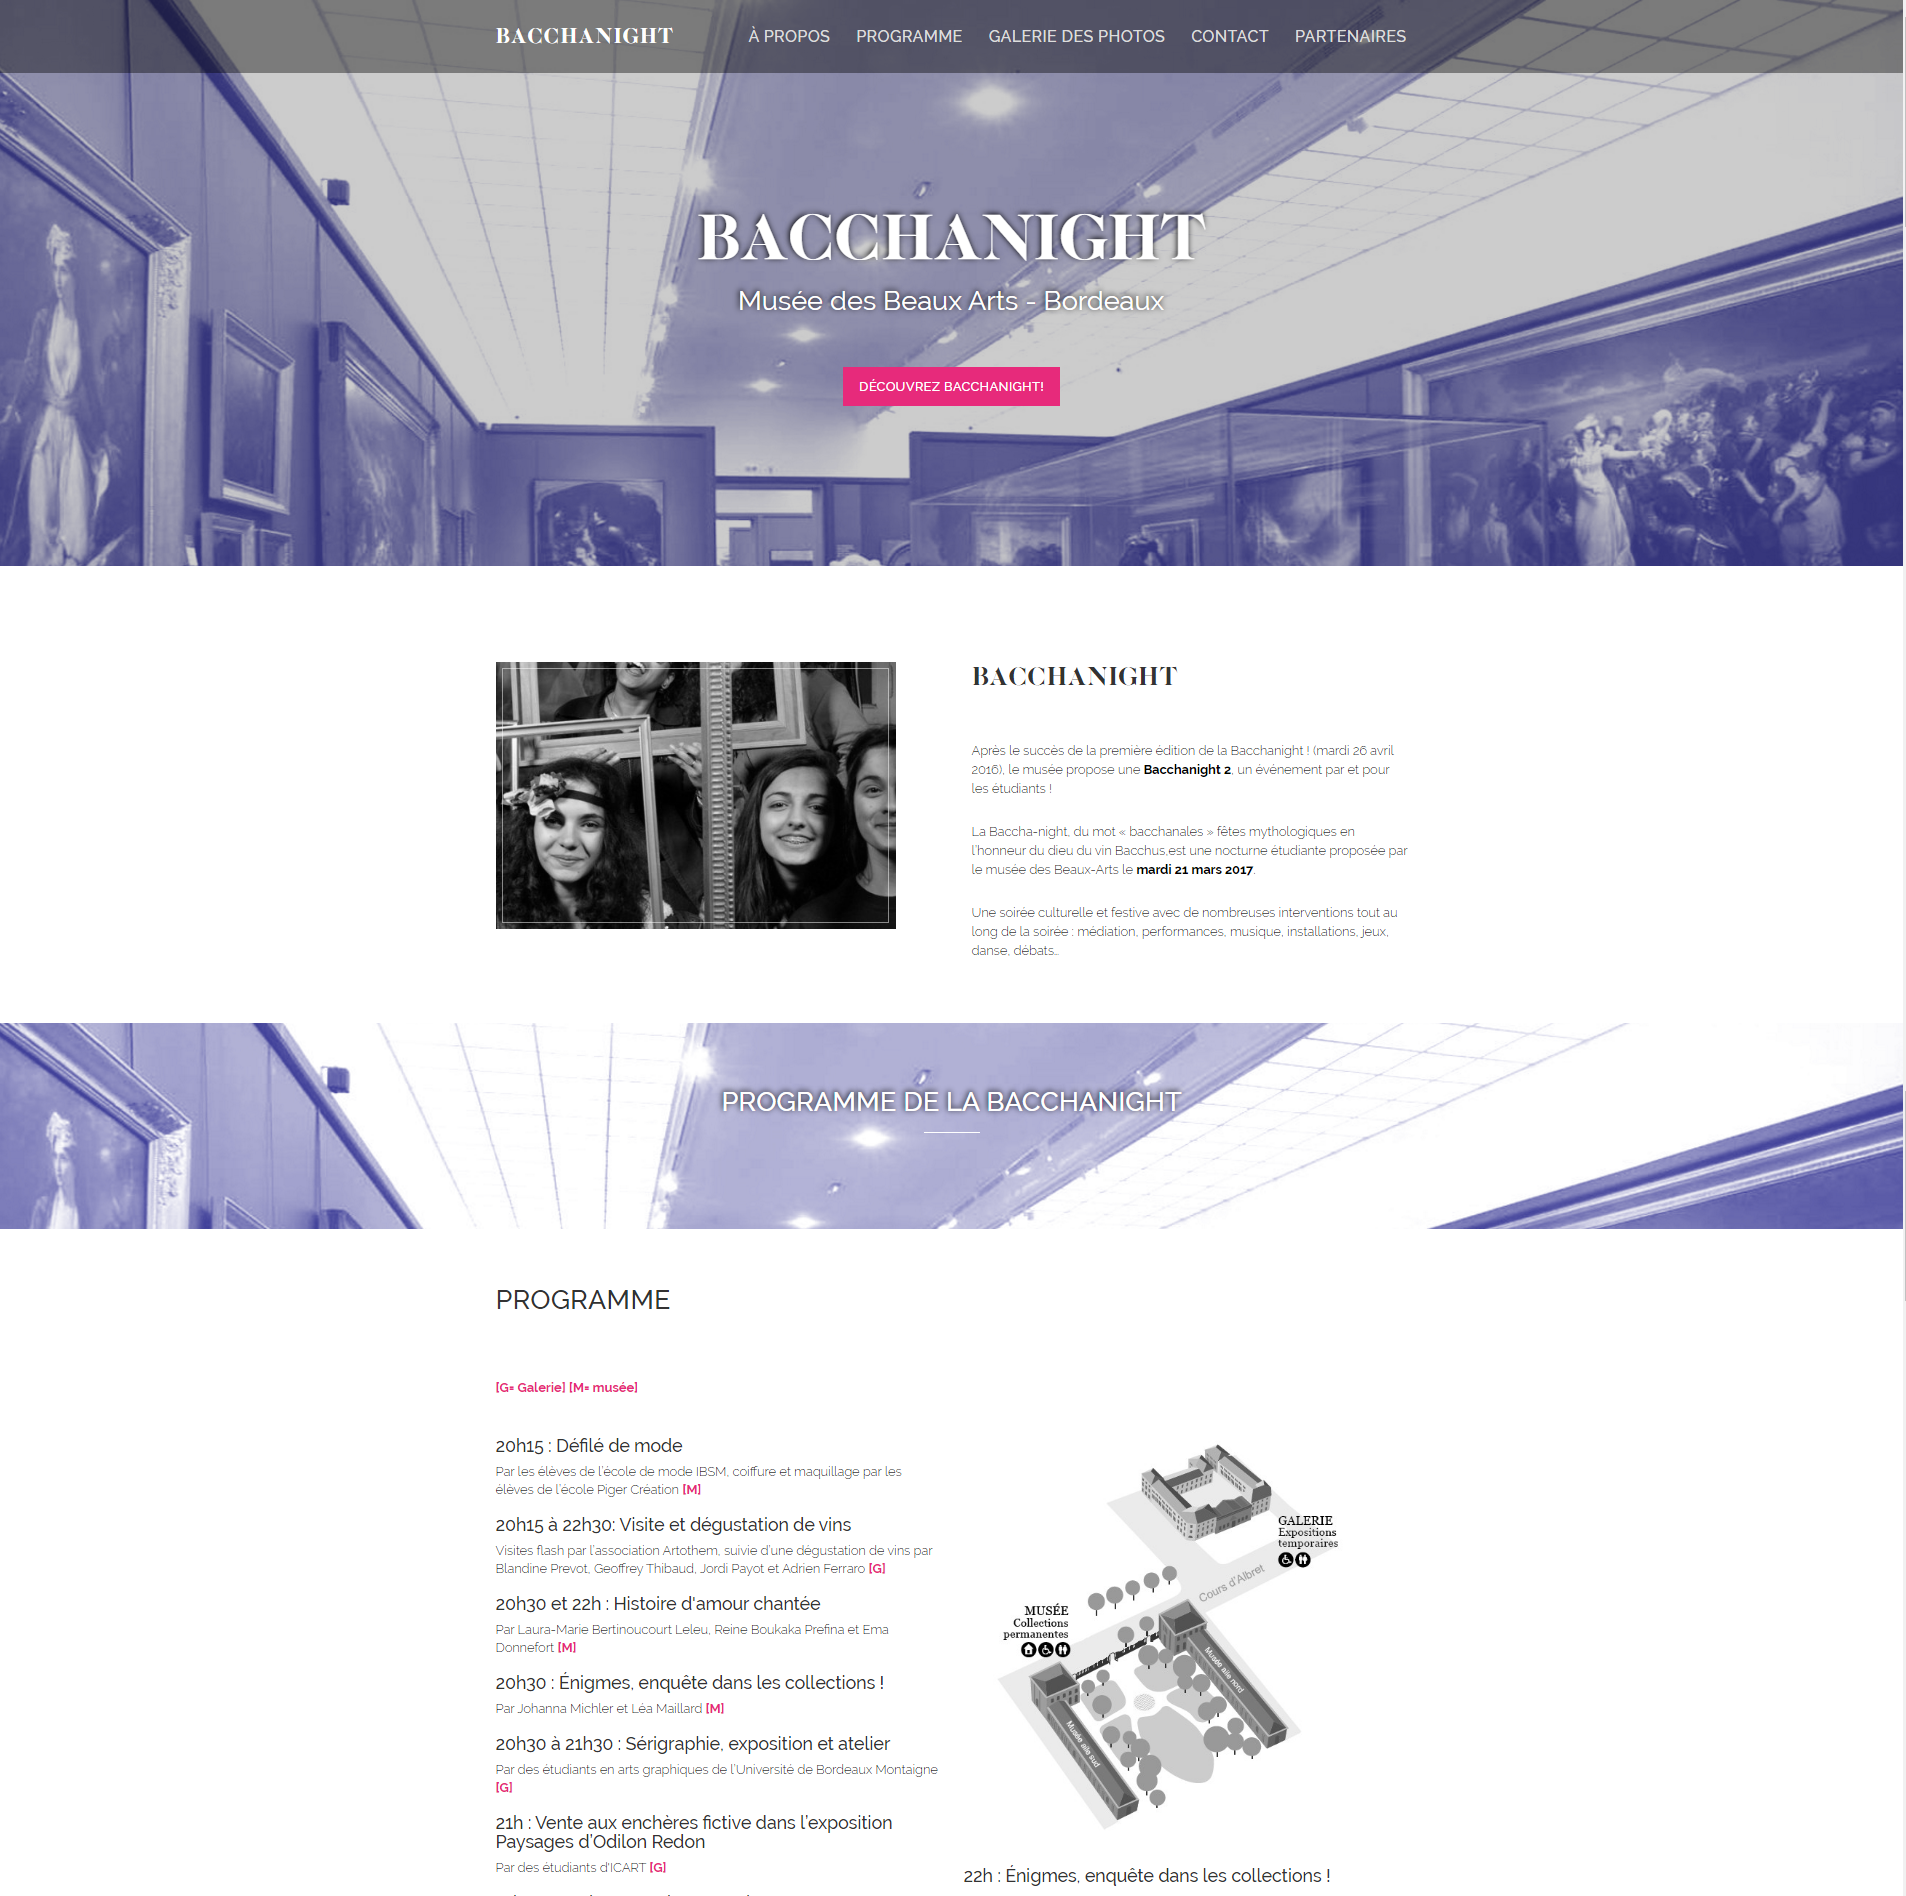
\includegraphics[width=\textwidth,height=\textheight,keepaspectratio]{preview2.png}

\end{document}
